\chapter{Technology of ice reservoirs}
\label{chap:tech}

\cleanchapterquote{In building ice stupas, it's necessary to engage enough workforce to extract the water over
  long distances and to keep water flowing in cold temperatures.}{Marcus Nüsser}{(Professor, South Asia Institute)}

There is a long tradition of developing ice harvesting structures in the upper Indus Basin, in both Ladakh,
northern India \citep{labbalTraditionalOasesLadakh2000, nusserIrrigationDevelopmentUpper2012} and various
locations in northern Pakistan \citep{kreutzmannScarcityOpulenceWater2011}. AIRs, located at much lower altitudes
than naturally occuring glaciers, serve to bridge the critical gap in water availability by providing
meltwater earlier in the agricultural season. Such ice reservoirs utilize the hydrological process of icing
under local conditions of frequent freeze-thaw cycles to capture water for seasonal storage. They are not water
storage structures that freeze from the top down, rather they are produced through sequential, freezing of thin
layers of water creating superimposed sheets of ice.

\begin{figure}[htb]
\centering
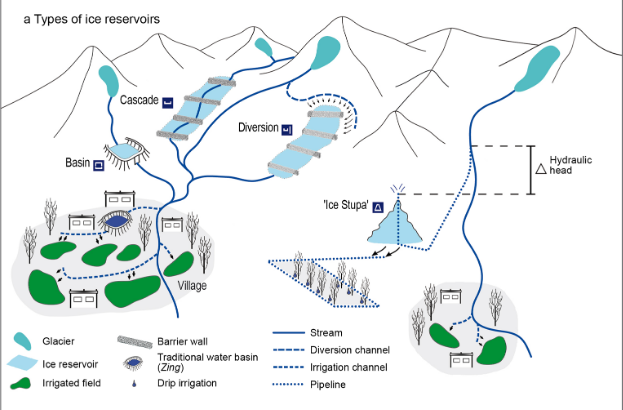
\includegraphics[width=\textwidth]{figs/AIR_designs}
\caption{Different types of ice reservoirs. Adapted from \cite{nusserSociohydrologyArtificialGlaciers2019}}
\label{fig:AIRdesigns}
\end{figure}

In this chapter, we present the various types of ice reservoirs that exist ( Fig. \ref{fig:AIRdesigns}),
describe their construction strategy and explore the benefits of automated construction strategies.


% \section{Traditional construction strategy}
\section{Types of ice reservoirs}

\subsection{Ice terraces}

According to oral history and corona imagery from 1969, the first ice terraces are older than 50 years and can
be found in Phuktse and Igoo villages of Ladakh. Over the past 30 years, 14 ice terraces have been constructed in central Ladakh,
located in tributary valleys of the Indus \citep{norphelArtificialGlacierHigh2009,
nusserSociohydrologyArtificialGlaciers2019}. Chewang Norphel, a well known engineer of the Leh Nutrition
Project, introduced this practice to Ladakh \citep{vinceGlacierMan2009}. Cascades and diversions shown in Fig.
\ref{fig:AIRdesigns} constitute the ice terrace type of AIRs.

\begin{figure}[htb]
\centering
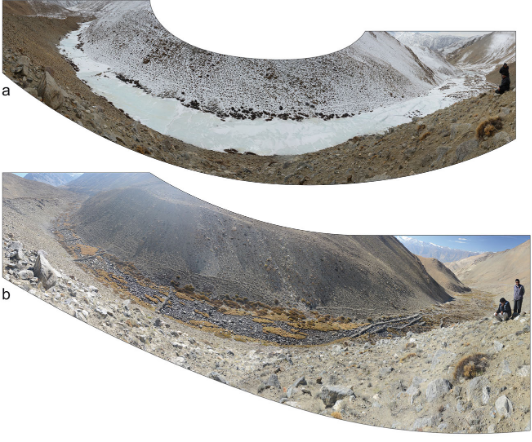
\includegraphics[width=\textwidth]{figs/IT_example.png}
\caption{Ice terrace of Phuktse, viewpoint 4430 m. (a) February 2014 (b) October 2014 Adapted from: \cite{nusserSociohydrologyArtificialGlaciers2019}}
\label{fig:ITexample}
\end{figure}

There are two distinct types of ice terraces with site-specific modifications as shown in Fig.
\ref{fig:AIRdesigns}: the first type is built as cascades on perennial streams. A series of loose rock walls in
the river bed reduces flow velocity, but still lets water pass through. Such cascades allow flowing water to
freeze on exposed surfaces and form superimposed ice layers when temperatures drop ( Fig.
\ref{fig:ITscience}). An example of this is illustrated in Fig. \ref{fig:ITexample}.

The second type diverts water from streams with higher flow velocity to small side valleys, shaded by
surrounding mountains. This design allows to integrate higher slope positions for additional ice formation. It
consists of a series of partially cemented stone walls across the stream bed. Their dimensions are adjusted
based on the valley topography. The water for the ice terrace is obtained through a long diversion channel.

\begin{figure}[htb]
\centering
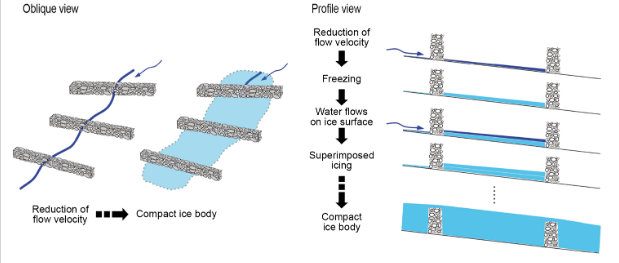
\includegraphics[width=\textwidth]{figs/IT_science.png}

\caption{ The process of ice accumulation for ice terraces. Adapted from
\citet{nusserSociohydrologyArtificialGlaciers2019}}

\label{fig:ITscience}
\end{figure}

The following construction guidelines are applied depending on the terrain of the construction site
\citep{norphelSnowWaterHarvesting2015}:

\begin{itemize}

  \item If the section of the stream is very wide with a mild slope, then stone walls are
    constructed in a series parallel to each other. The number and dimension of ice-retaining walls depend on
    the flow of water available in the main stream during peak winter.

  \item If the section of the stream is narrow with a steep gradient then it needs to be diverted to a shady area
    by constructing a gravitational channel with sufficient slope. When it reaches the ice terrace site the
    inclination should be gradually reduced, allowing the water to flow through small outlets thus accelerating freezing. Stone
    walls need to be constructed parallel to the channel in series, according to the natural slope of the terrain.
    The steeper the terrain, the smaller the distance and slope between the bunds.

\end{itemize}


\subsubsection{Water storage and cost}

The volume variations of ice terraces within Ladakh range from 510 $m^3$ to 81,040 $m^3$ highlighting
the importance of local topography and microclimate in their formation
\citep{nusserSociohydrologyArtificialGlaciers2019, norphelSnowWaterHarvesting2015}. The cost of construction
depends on the size and number of stone walls required. The estimated material cost of ice terraces vary between
4600 to 15,330 USD \citep{nusserSociohydrologyArtificialGlaciers2019}. The building of ice terraces also relies
on the participation of village communities for construction and maintenance. 

\subsection{Ice stupas}

\begin{figure}[htb]
\centering
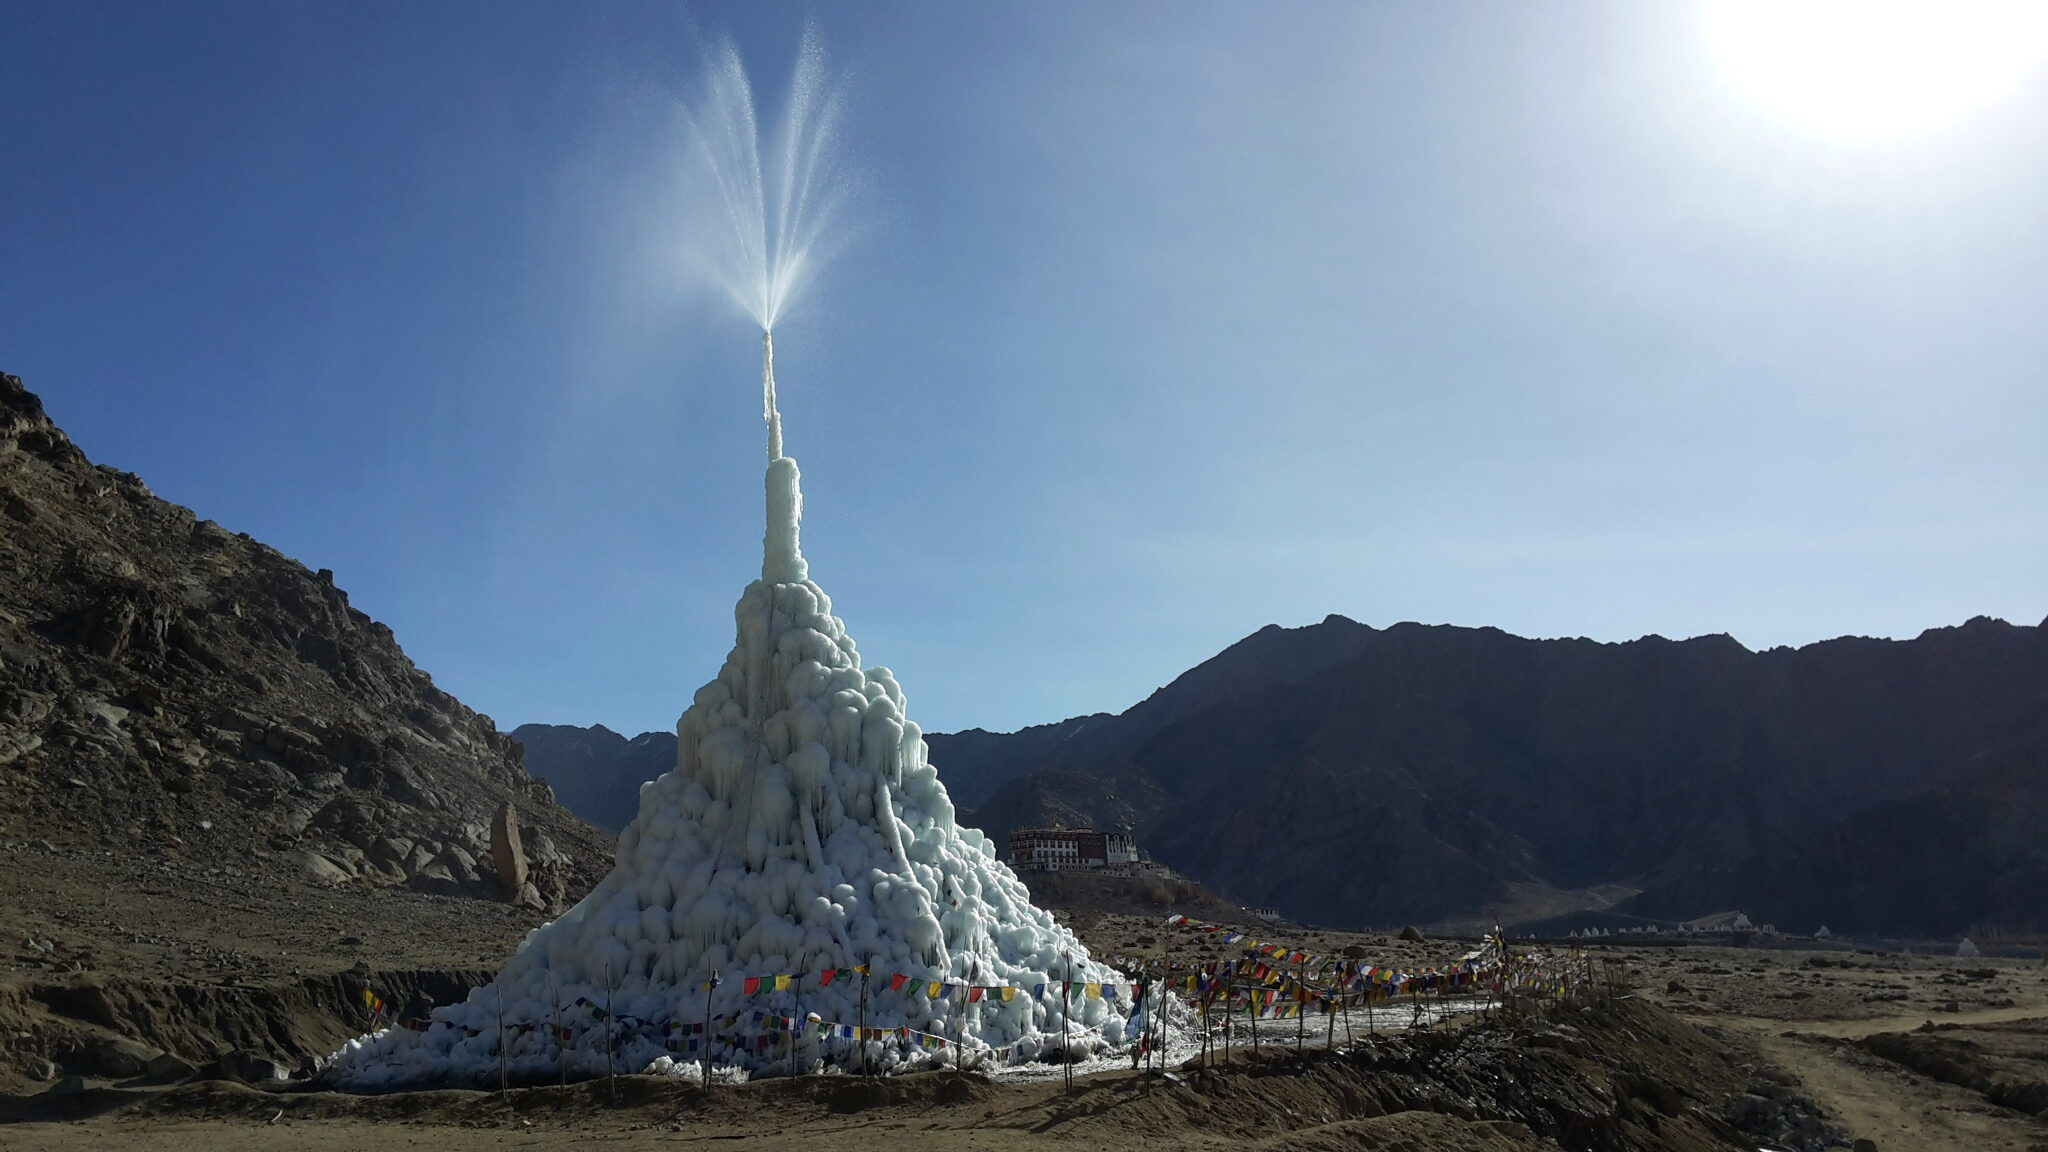
\includegraphics[width=\textwidth]{figs/IS_example.jpg}
\caption{Ice stupa of Phyang village on March 2015.}
\label{fig:ISexample}
\end{figure}

Ice stupas, invented by Sonam Wangchuk in 2013, provide a much easier way to achieve water storage compared to
ice terraces \citep{wangchukIceStupaArtificial2014}. Ice stupas can be placed much closer to the plantations
since they absorb less solar radiation per unit of volume compared to ice terraces due to their conical shape.
However, the typical volume range of ice stupas is also much smaller than that of ice
terraces \citep{nusserSociohydrologyArtificialGlaciers2019}. Over the past decade, several ice stupas have been
built to supplement irrigation water supply of mountain villages in India
\citep{wangchukIceStupaCompetition2020, palmerStoringFrozenWater2022, aggarwalAdaptationClimateChange2021},
Kyrgyzstan \citep{bbcnewsBrightArtificialGlacier2020}, Nepal and Chile
\citep{reutersConservationistsChileAim2021}.


\begin{figure}[htb]
\centering
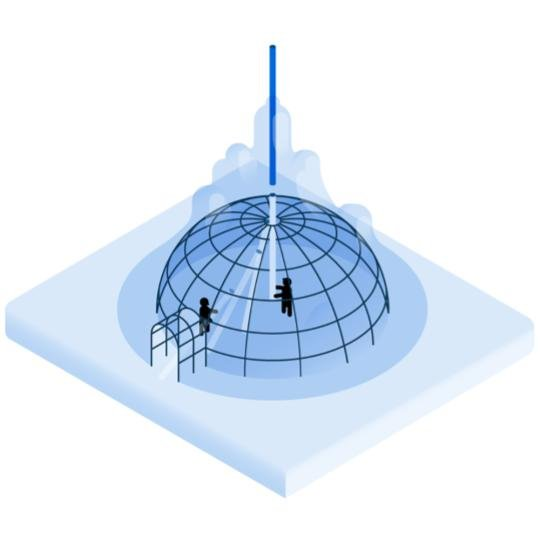
\includegraphics[width=8cm]{figs/IS_science.jpg}
\caption{The construction process of ice stupas. Diagrams by: Francesco Muzzi }
\label{fig:ISconstruction}
\end{figure}

A typical ice stupa simply requires a fountain nozzle mounted on a supply pipeline (Fig. \ref{fig:ISexample}).
The water source is usually a glacial stream. Due to the altitude difference between the pipeline input and
fountain output, water ejects from the fountain nozzle as droplets which freeze under subzero winter conditions.
The fountain is manually activated during winter nights. The fountain nozzle is raised through the addition of
metal pipes when significant ice accumulates below (Fig. \ref{fig:ISconstruction}). Typically, a dome of
branches is constructed around the metal pipes so that pipe extensions can be installed from within this dome.
Threads, tree branches and fishing nets are used to guide and accelerate the ice formation.

\subsubsection{Water storage and cost}

\begin{figure}[htb]
\centering
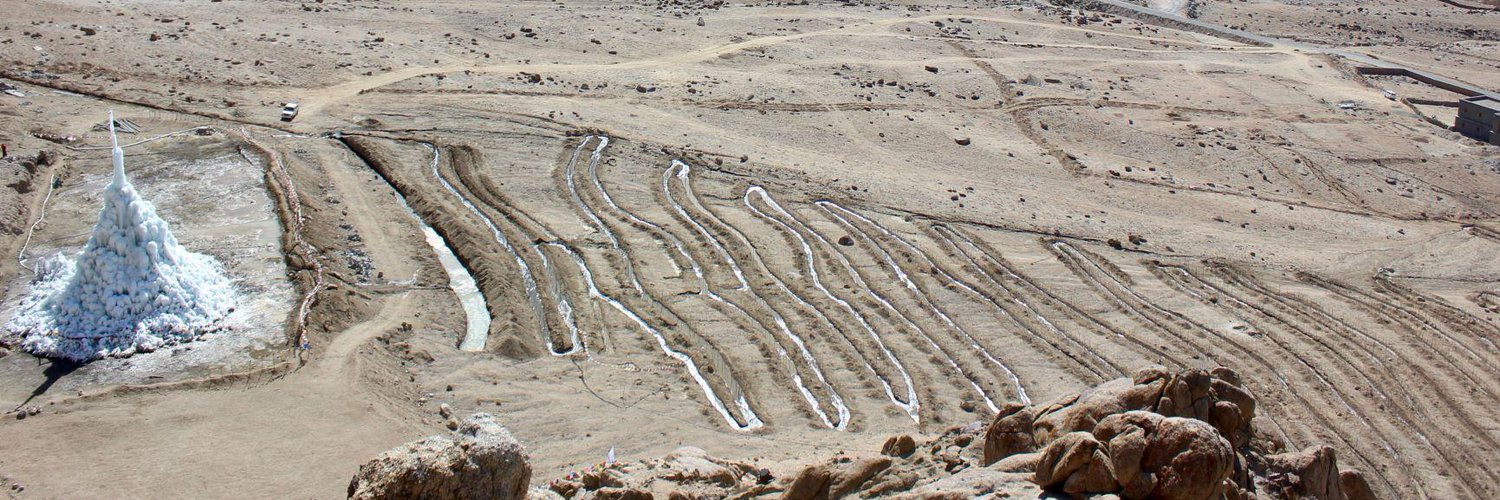
\includegraphics[width=\textwidth]{figs/IS_irrigation.jpeg}
\caption{Irrigation channel of the ice stupa at Phyang village. (P.C. Lobzang Dadul) }
\label{fig:ISirrigation}
\end{figure}

\begin{figure}[htb]
\centering
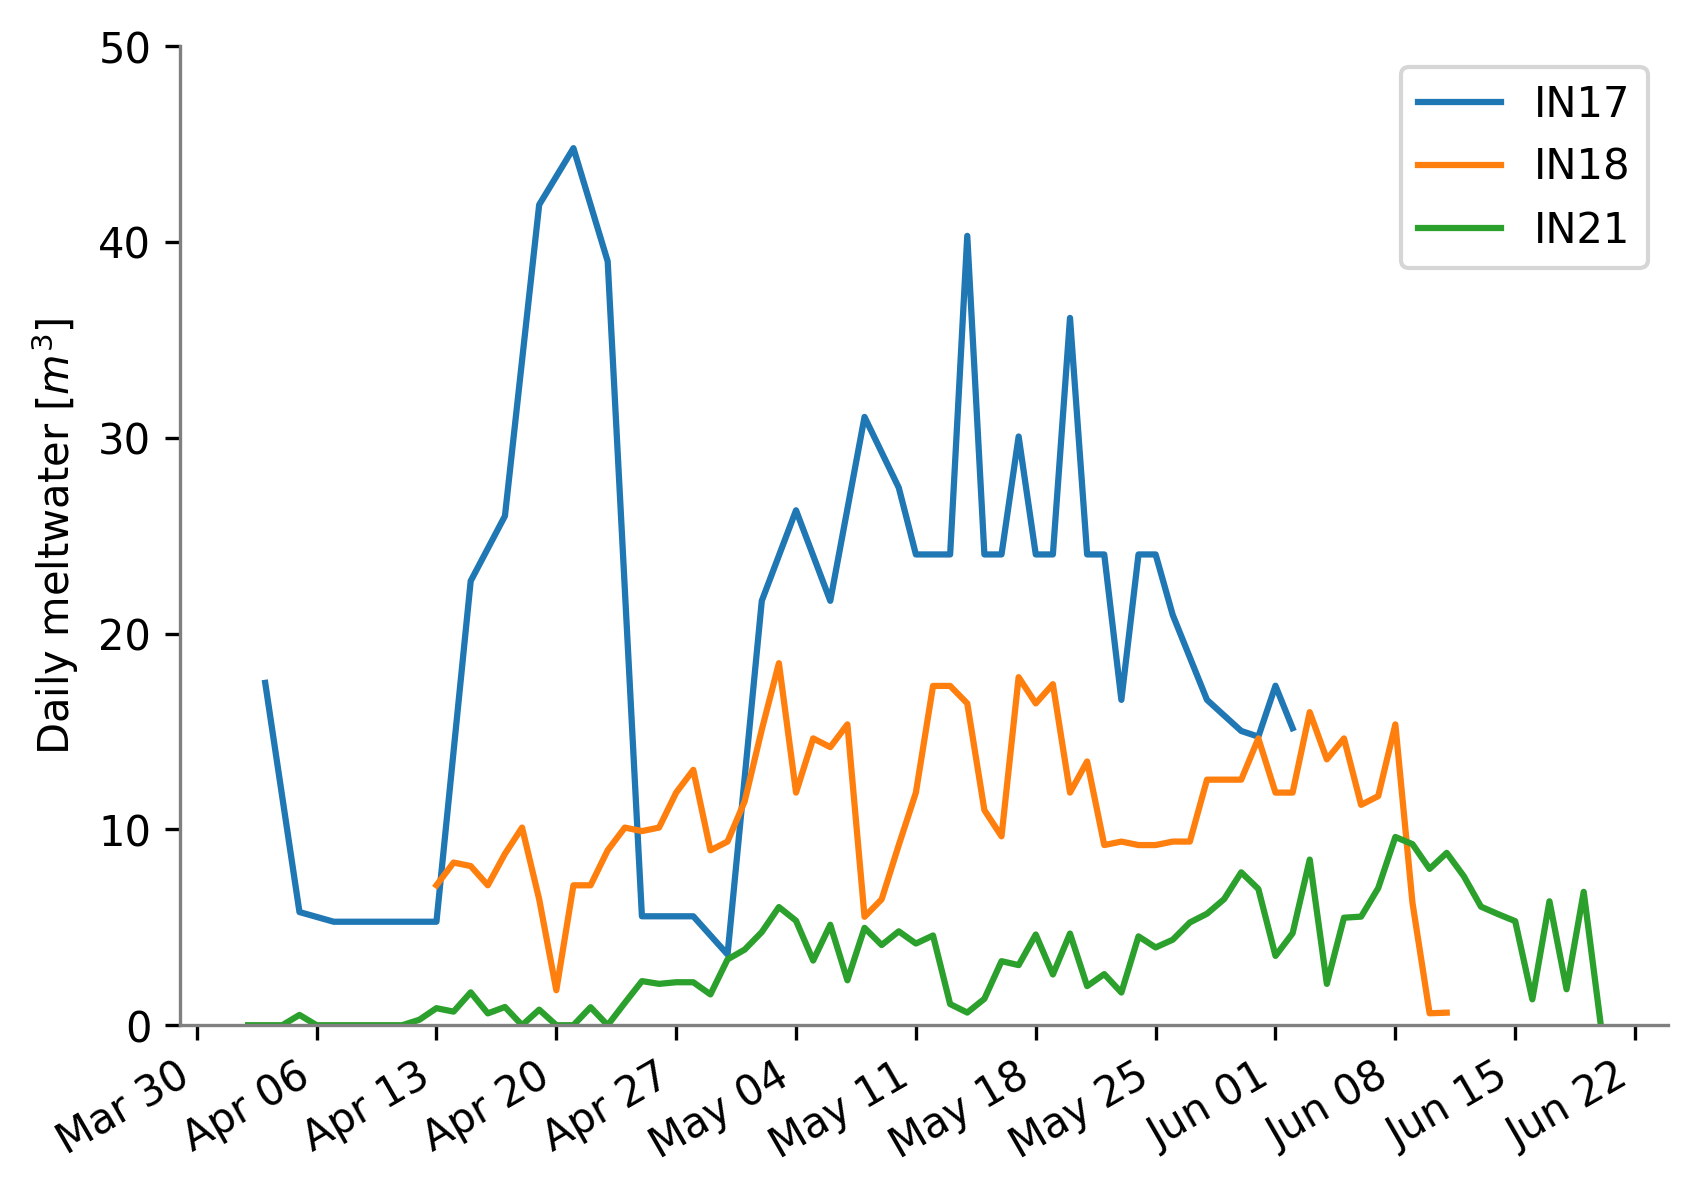
\includegraphics[width=\textwidth]{figs/melt.png}
\caption{Daily meltwater measurements for the IN17 and IN18 AIRs along with the corresponding model estimations
for the IN21 AIR. }
\label{fig:ISmelt}
\end{figure}

The cost of construction primarily depends on the material, size and length of the pipeline required. The
fountain nozzle's cost is negligible in comparison. Typical pipeline configuration in Ladakh consists of a high
density polyethylene pipeline of 63 $mm$ diameter. The estimated cost of such a pipeline system is around 6,875
USD per $km$ of pipeline length.

Figure \ref{fig:ISmelt} shows the temporal variation of daily meltwater quantities obtained from 3 different
AIRs built in Ladakh during their melting periods (mid-April to mid-June). IN17 and IN18 AIRs were constructed
in Phyang village and their meltwater quantities were measured manually (Fig. \ref{fig:ISirrigation}). These
measurements were performed by recording the water level of a icestupa meltwater collection tank
\citep{simantvermaIceStupaMeltwater2018}. IN21 was constructed in Gangles village and its meltwater quantities
were modelled. The differences between the AIRs reflect the corresponding interannual variability in the weather
conditions. The median daily AIR meltwater quantities measured were higher than 11 thousand litres. 

\section{The need for water supply management}

A common issue of AIR construction systems is water supply management, namely answering the questions "when to
water?", "how much?", and "for how long?". Starting water supply too early, spraying too much water, or
running water supply for too long might lead to overwatering; at the very least, this practice wastes water.
Similarly, starting the water supply too late, supplying too little water, or not running the water supply long
enough might lead to underwatering and can cause reduced ice volume. The management of water supply
differs based on the type of the AIR used. In the following analysis, we restrict ourselves to the ice stupa
form of AIRs where water supply management can also be referred to as fountain scheduling.

Paper I has shown that traditional ice stupa construction systems suffer from overwatering. For example, in
Indian AIRs, the fountain discharge rate could theoretically be halved since it is always twice as high as the
modelled freezing rate. However, in practice, the reduction of discharge rate could increase maintenance costs
due to higher risk of freezing events in the fountain pipeline.

An optimum construction strategy, therefore, should first prevent the occurrence of freezing events in the
fountain pipeline. These events can be prevented by setting a minimum threshold for the recommended discharge
rate. The discharge scheduler software developed in the previous chapter satisfies these requirements.

Adjusting the fountain discharge rate manually is not practical due to two reasons: first, this would involve
constant adjustments of discharge rates in response to the significant diurnal and seasonal variations of the
freezing rates; second, frequent pipeline water drainage would be required to avoid water losses. Therefore, operation
of scheduled fountains via automation systems is preferred to reduce long-term maintenance costs. The
hardware used to implement such an automation system is described in paper II.

This section aims to compare the water-use efficiency, maximum ice volume and maintenance effort between
traditional and automated construction strategies. First, two AIRs were built in the same location but with and
without automated fountain scheduling strategies; both were measured and compared (Fig. \ref{fig:autovsman}).
The associated datasets and the methods used to analyze them are described in paper II. In a second step,
differences in construction strategies between the Indian and Swiss AIRs studied in previous winters were quantified
using model simulations. Later we discuss how these construction strategies can help scale the ice volumes and
survival duration of AIRs. 

\begin{figure}[htb]
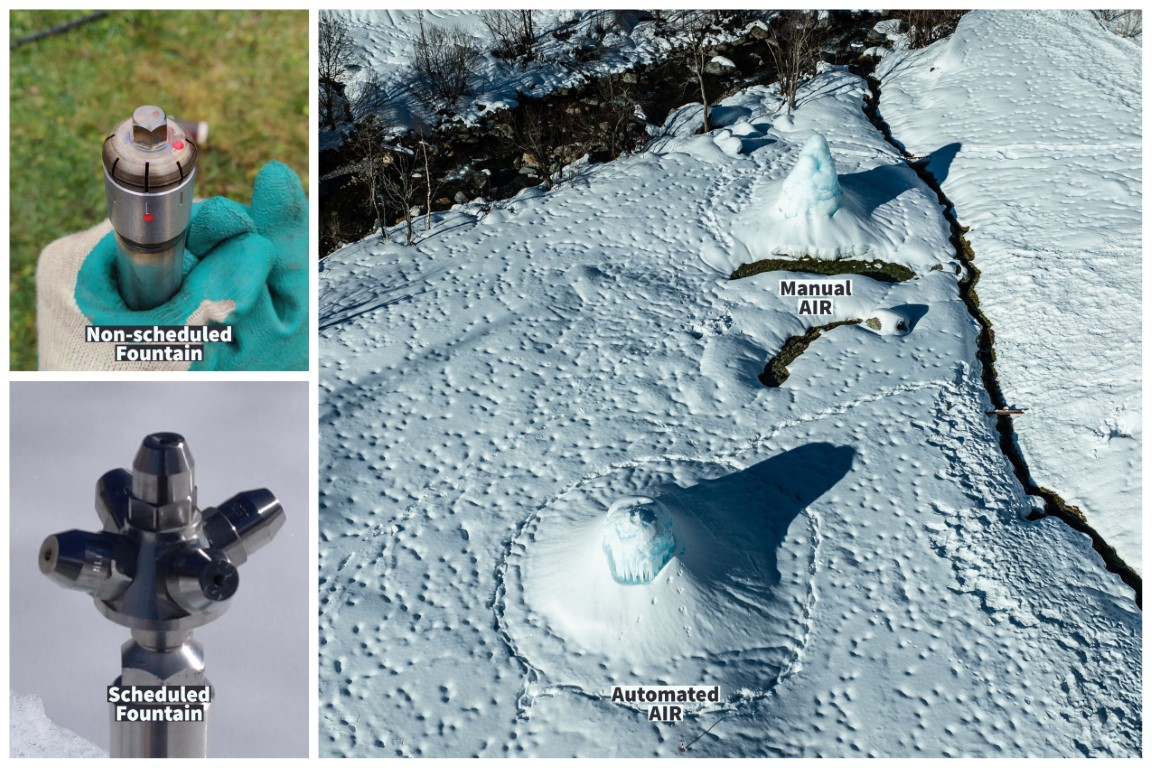
\includegraphics[width=\textwidth]{figs/AIR_fountains.jpg}
\caption{Unscheduled and scheduled fountains used for construction of traditional and automated AIRs at Guttannen. Picture credits: Daniel Bürki}
\label{fig:autovsman}
\end{figure}

\subsection{Automated fountain scheduling system}


Recommended discharge rates can only be produced if more information about the AIR surface properties and
weather conditions are available. Particularly, resolving the uncertainty in the expected freezing rate requires
quantification of the following three model variables: slope, albedo and cloudiness. But these properties cannot
be predicted beforehand. Therefore, we instead associate the upper and lower bound of each variable to a
different model depending on whether they increase the freezing rate or not. Higher slope and albedo values
decrease the shortwave radiation impact. Higher cloudiness values increase both the shortwave and the longwave
radiation impact. The model overestimating the freezing rate will be referred to as \ac{IVOM} and the model
underestimating the freezing rate will be referred to as  \ac{WEOM}, respectively. Accordingly, the values
assigned for all the three variables in the respective model is shown in Table \ref{tab:assumptions}.

The fountain scheduling software implements two types of fountain scheduling strategies depending on which
model type is suitable. WEOM model type is used if the location has limited water availability since it is expected to
produce better water-use efficiency. \ac{IVOM} model type is used if the location had limited duration of favourable
weather windows since it is expected to produce higher ice volumes. These two kinds of scheduled fountains will
be referred to as water-sensitive fountain and weather-sensitive fountain henceforth.

\begin{table}[htb]
\centering
\caption{Assumptions for the parametrisation introduced to simplify the ice volume optimised model (IVOM) and
water-use efficiency optimised model (WEOM). $\alpha_{snow/ice}$ represents albedo of snow or ice respectively.}
\label{tab:assumptions}
\begin{tabular}{|lllll|}
\toprule
\textbf{Estimation of} & \textbf{Symbol} & \textbf{IVOM} & \textbf{WEOM} & \\\midrule
\multicolumn{1}{|l}{Slope}        & $s_{cone}$ & 1 & 0 & \multicolumn{1}{l|}{} \\ 
\multicolumn{1}{|l}{Albedo} & $\alpha$ & $\alpha_{snow}$ & $\alpha_{ice}$ & \multicolumn{1}{l|}{} \\
\multicolumn{1}{|l}{Cloudiness}  & $cld$ & $0$ & $1$ & \multicolumn{1}{l|}{} \\\bottomrule 
\end{tabular}
\end{table}

We apply the assumptions described in Table \ref{tab:assumptions} on the one-dimensional description of energy
fluxes through Eqn. \ref{eqn:EB}. The derivation of the individual energy and mass balance terms for the
\ac{IVOM} and \ac{WEOM} model versions are discussed in the Appendix \ref{sec:auto_software}.

Equation \ref{eqn:EB} is implemented in the automation software. The user interface of the software enables
input of the spray radius, altitude, latitude and longitude of the construction location. The automation
hardware consists of an AWS, flowmeter, control valve, drain valves, air valves, fountain, pipeline and a
logger. The logger feeds the AWS data to the automation software and informs the recommended discharge rate to
the flowmeter. The flowmeter adjusts the control valve to match the recommendation. When a termination
criteria is met, the drain and air valves allow the removal of water from the pipeline and the entry of
air in the pipeline respectively.

The recommended discharge rate is equal to the mass change rate. However, certain termination criteria listed
below override the discharge rate recommendation and drain the pipeline to prevent water loss or fountain
freezing events:

\begin{itemize}

\item High water loss is assumed if wind speed is greater than the user-defined critical wind speed.

\item High risk of fountain freezing event is assumed if mass change rate is lower than the user-defined minimum fountain discharge rate. 

\item Freezing events in the fountain pipeline are assumed if measured discharge rate is zero for at least 20
  seconds. 

\item Pipeline leakage is assumed if measured discharge rate is greater than the user-defined maximum fountain discharge rate.

\end{itemize}

\subsection{Comparison of traditional and automated construction strategies}

\begin{figure*}[htb] 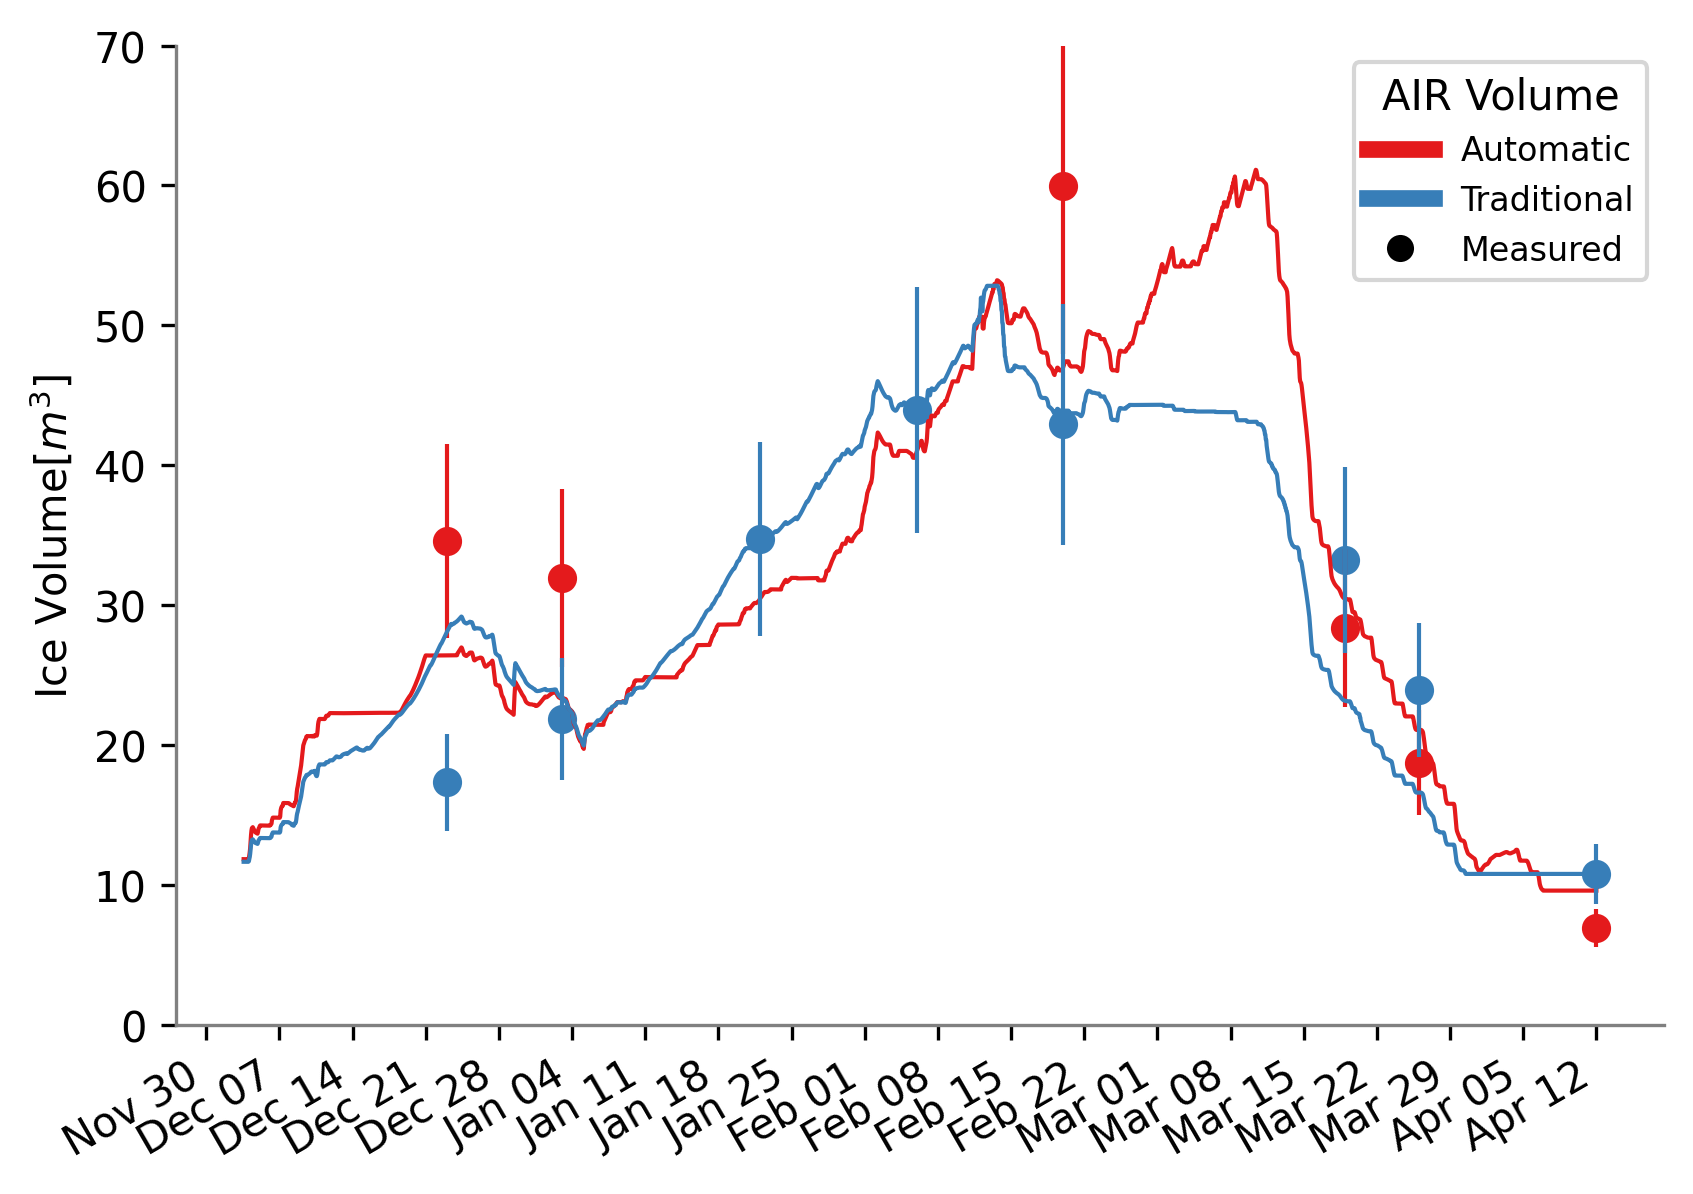
\includegraphics[width=\textwidth] {figs/CH_validation.png} \caption{Volume validation of the
scheduled and unscheduled fountain construction strategies.} \label{fig:validation} \end{figure*}

Fountain scheduling reduced the fountain discharge input and fountain wastewater output by an order of
magnitude. However, this does not result in an appreciable difference in the volume evolution of the automated
or traditional AIR, as shown in Fig. \ref{fig:validation}. This is due to two counteracting surface processes
during fountain spray: process A consists in the dampening of albedo to ice albedo and process B consists in the
absorption of heat energy from the fountain water droplets. The temporal variation of the magnitude of these
processes is shown in Fig. \ref{fig:dis_processes}.

\begin{figure*}[htb]
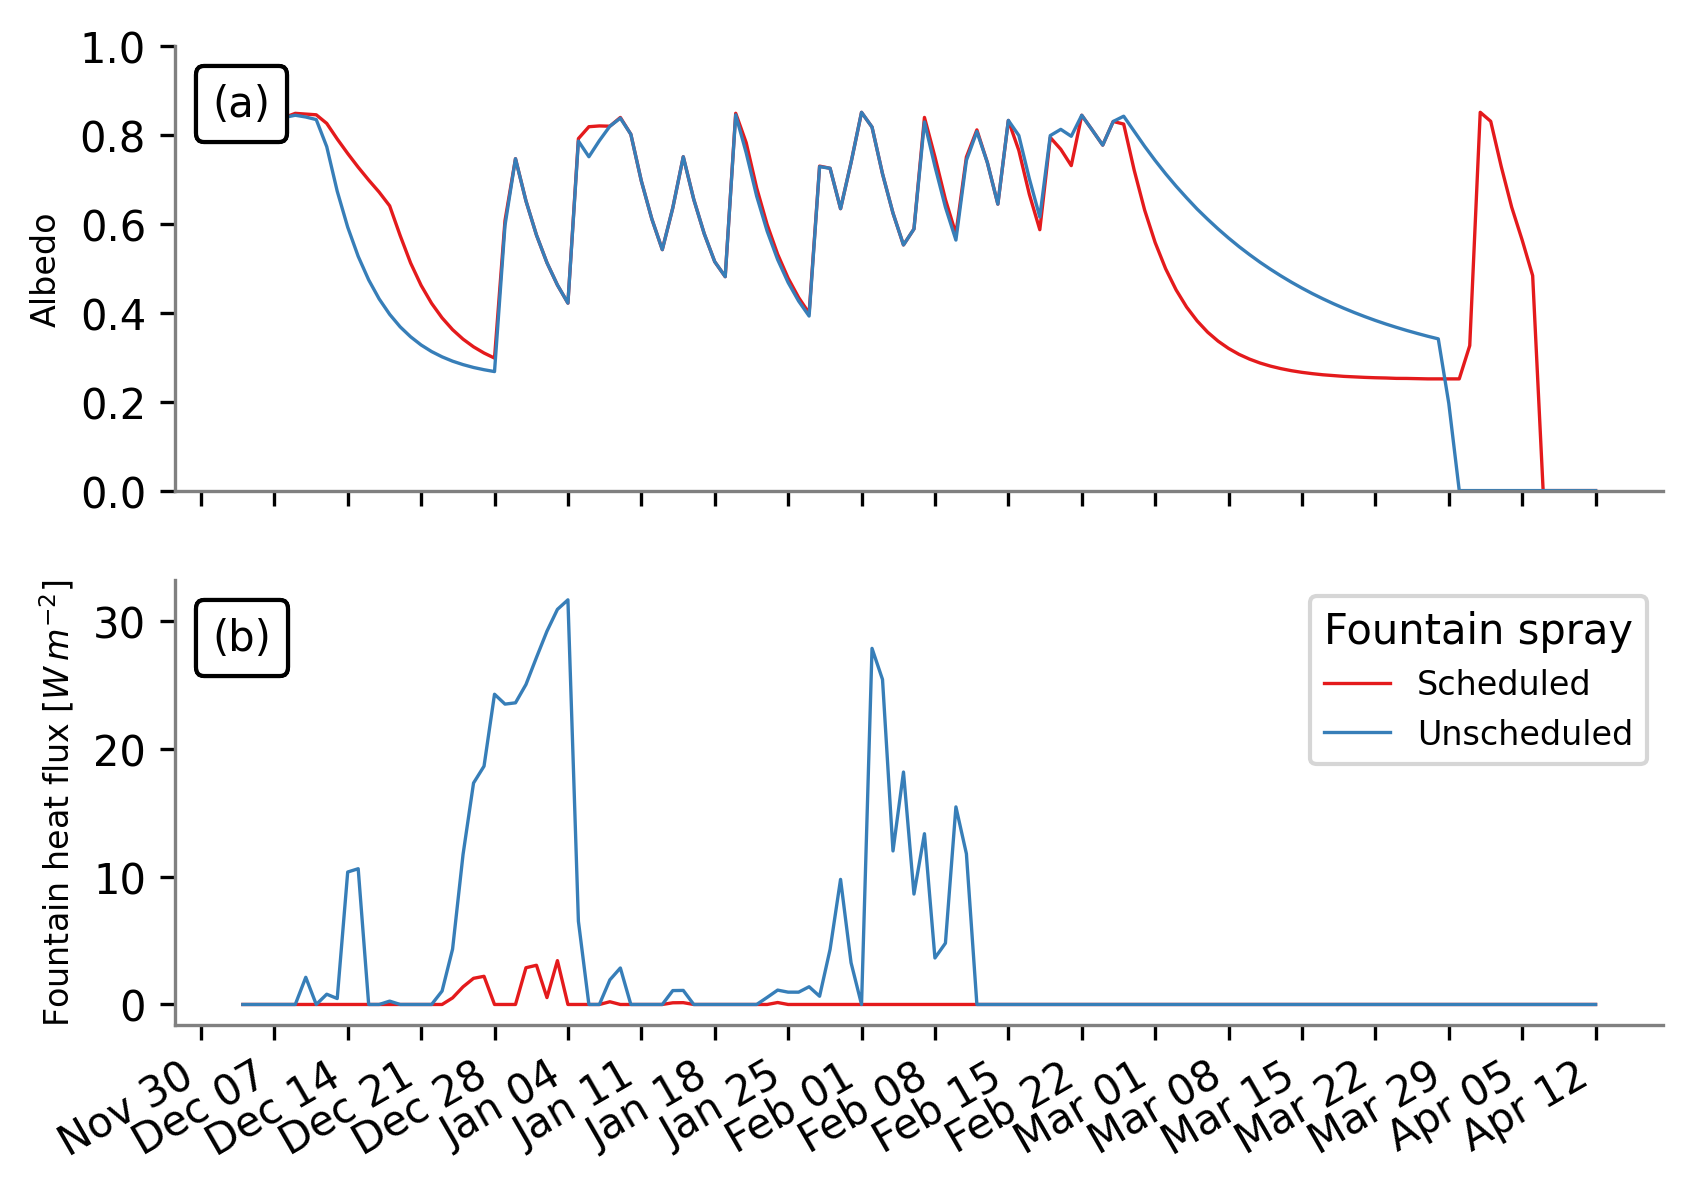
\includegraphics[width=\textwidth]{figs/dis_processes.png}
\caption{(a) Surface albedo  and (b) fountain discharge heat flux showed significant variations between the two
  AIRS due to the differences in their discharge rates.}
\label{fig:dis_processes}
\end{figure*}

The difference in water-use efficiency and maximum ice volume between unscheduled and scheduled fountains in the
Indian and Swiss locations across two winters is shown in Fig. \ref{fig:wue}a. Four experimental values
(highlighted in circles) and five simulated values (highlighted in squares) are shown together.  The
experimental values were taken from the IN21 and CH21 AIRs studied in paper I and the CH22 AIR investigated in
paper II. 

\begin{figure}[htb]
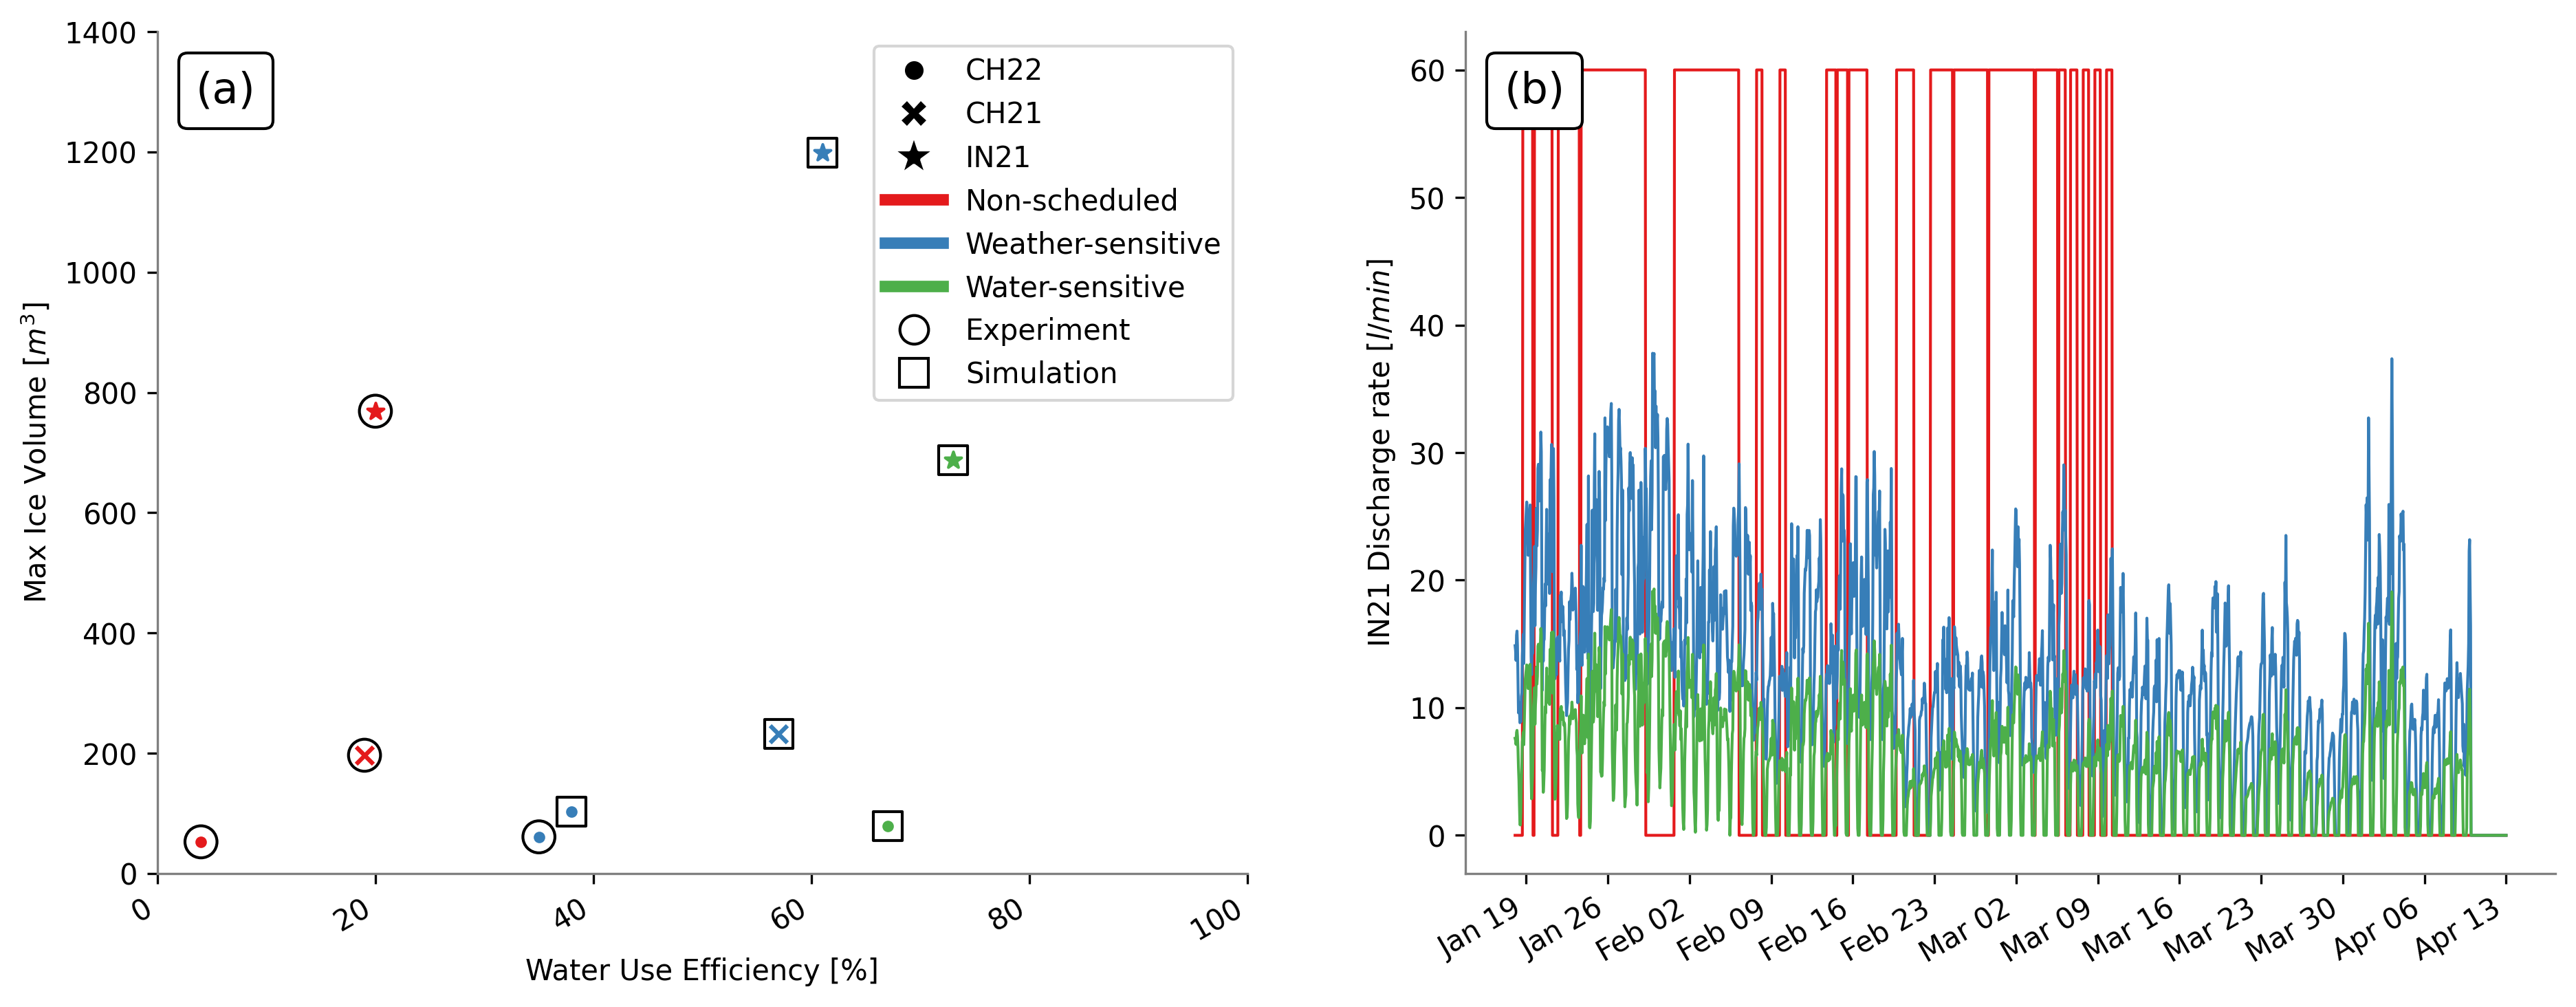
\includegraphics[width=\textwidth]{figs/wue.png}

\caption{(a) The maximum volume and water-use efficiency estimated for AIRs constructed in different locations
(represented by symbols) with different fountain scheduling strategies (represented by colours). Experimental
values are highlighted in circles and simulated values are highlighted in squares. (b) Comparison of
the unscheduled and scheduled fountain discharge rates at the IN21 location.}

\label{fig:wue}
\end{figure}

The water-use efficiency of all the unscheduled fountains is below 20 \%. In general, water-use efficiency
exhibits a threefold increase when the weather- or water-sensitive fountains are used in both
locations.  

For the Indian location, the three different kinds of fountains yielded significantly different results owing to discharge
duration and max discharge rate
(Fig. \ref{fig:wue}b). The unscheduled fountain showed a maximum discharge rate more than twice that of
the scheduled fountains, resulting in higher water loss; freezing events in its pipeline caused frequent
interruptions in the unscheduled discharge rate (Fig. \ref{fig:wue}b). In contrast, the mean freezing
rates of the other two fountains during these events were above their median values. This is because very cold
temperatures freeze the water inside rather than outside the fountain system, instigating such freezing events in
the fountain pipeline. Therefore, the discharge duration of the unscheduled fountain was much lower, resulting in
lower ice volume. The water-sensitive fountain underestimated the freezing rate during the construction period
and therefore produced much lower ice volume compared with the weather-sensitive fountain. 

For the Swiss locations, scheduled fountains yielded better water-use efficiency but did not significantly alter the maximum
volume obtained. 

